\documentclass[12pt]{article}

\usepackage{sbc-template}
\usepackage{graphicx,url}
\usepackage[utf8]{inputenc}
\usepackage[brazilian]{babel}
\usepackage{amsmath}
\usepackage{booktabs}

\sloppy

\title{GhostPredict: uma prova de conceito de compressão sem perdas\\
com prior embutido no codec para micro-payloads de IoT}

\author{Matheus Araújo\inst{1}}

\address{Projeto de pesquisa independente
  \email{araujomatheuscarv@gmail.com}
}

\begin{document}

\maketitle

\begin{abstract}
  General purpose compressors such as gzip, zstd and brotli enlarge very short
  messages, because header and framing overhead exceeds any saving. This work
  presents GhostPredict, a proof of concept of a lossless compressor for the
  micro-payloads of tens of bytes that dominate IoT telemetry, built to test
  whether a domain prior shared in the codec, rather than in the file, pays off
  in this regime. The method combines a header free
  format, an order-2 context model over nibbles with integer arithmetic coding,
  and a domain prior embedded in the codec rather than in the file, which warms
  the statistical model and acts as an LZ dictionary. Across eleven real
  datasets the primed variant produces the smallest file in 94\% to 100\% of
  the messages; once the removable dictionary framing is discounted, the
  reduction factor over the lean zstd dictionary averages 1.73. We quantify the
  dependence on a domain matched prior, translate byte savings into LoRaWAN
  time on air and transmission energy, and report on-target measurements on an
  ESP32, where the decoder uses 19,692 bytes of static RAM and 698 microseconds
  per message without the prior, and 47.7 milliseconds with it. The results
  support the feasibility of the approach and identify the steps still needed
  for production use.
\end{abstract}

\begin{resumo}
  Compressores de propósito geral como gzip, zstd e brotli aumentam o tamanho
  de mensagens muito curtas, pois o custo de cabeçalho e enquadramento supera
  qualquer economia. Este trabalho apresenta o GhostPredict, uma prova de
  conceito de compressor sem perdas para os micro-payloads de dezenas de bytes
  da telemetria de IoT, construída para verificar se um prior de domínio
  compartilhado no codec, e não no arquivo, compensa nesse regime. O
  método combina um formato sem cabeçalho, um modelo de contexto de ordem 2
  sobre nibbles com codificação aritmética inteira, e um prior de domínio
  embutido no codec, e não no arquivo, que aquece o modelo e serve de
  dicionário. Em onze conjuntos de dados reais, a variante com prior produz o
  menor arquivo em 94\% a 100\% das mensagens; descontado o enquadramento
  removível do dicionário, o fator de redução sobre o zstd enxuto é de 1,73 em
  média. Quantificamos a dependência de um prior casado com o domínio,
  convertemos a economia em tempo de antena e energia no LoRaWAN, e relatamos
  medições em um ESP32, no qual o decodificador ocupa 19.692 bytes de RAM
  estática e 698 microssegundos por mensagem sem o prior, e 47,7 milissegundos
  com ele. Os resultados sustentam a viabilidade da abordagem e indicam as
  etapas que ainda faltam para uso em produção.
\end{resumo}

% ======================================================================
\section{Introdução}

A expansão da Internet das Coisas multiplicou um tipo de tráfego que os
compressores clássicos atendem mal: mensagens curtas, frequentemente de trinta
a uma centena de bytes, emitidas por sensores, rastreadores e dispositivos de
telemetria.\footnote{Assistentes de inteligência artificial baseados em modelos
de linguagem foram utilizados neste trabalho como ferramenta de consulta, para
levantamento e checagem de trabalhos relacionados, revisão de texto e de código,
sugestão de análises e discussão de decisões de projeto. Todos os números
apresentados foram produzidos pela execução dos programas descritos no artigo,
sobre os conjuntos de dados citados, e conferidos pelo autor, a quem cabe a
responsabilidade pelo conteúdo. O código e os dados que permitem refazer cada
medição estão no repositório público indicado ao final desta seção.}
Protocolos como MQTT e CoAP, e enlaces de baixa potência como LoRaWAN e NB-IoT,
transportam esse tipo de payload, no qual cada byte transmitido tem custo direto
em energia, em tempo de antena e em limites regulatórios de ciclo de trabalho.

Nesse regime de tamanho, os compressores de propósito geral tendem a aumentar o
dado em vez de reduzi-lo. Formatos como o DEFLATE \cite{deutsch:96}, o Zstandard
\cite{collet:21} e o Brotli \cite{alakuijala:16} carregam cabeçalhos, somas de
verificação e estruturas de bloco cujo custo fixo domina quando a entrada tem
poucas dezenas de bytes. Medimos esse efeito na Seção~\ref{sec:resultados}: em
seis dos onze domínios avaliados, o gzip aumenta mais de 88\% das mensagens, e o
xz aumenta praticamente todas.

Este trabalho investiga, por meio de uma prova de conceito, se um compressor
desenhado para esse nicho reverte o quadro. A proposta, chamada GhostPredict,
não é apresentada como produto acabado, mas como instrumento para testar essa
hipótese em dados reais e em hardware. Ela parte de três decisões de projeto: um
formato sem cabeçalho, em que o arquivo é apenas o fluxo aritmético; um prior de
domínio embutido no próprio codec, e não no arquivo, que aquece o modelo
estatístico e fornece um dicionário inicial, eliminando o custo de partida a
frio; e uma garantia de que nenhuma entrada é expandida além de margem
declarada.

É legítimo perguntar, desde já, em que a proposta difere de um dicionário
externo, recurso que o zstd oferece de forma madura com dicionários treinados. A
diferença está em três pontos verificáveis. Primeiro, o formato: mesmo com
dicionário, cada quadro do zstd carrega um enquadramento fixo, que em nossa
variante mais enxuta ainda soma nove bytes, custo proporcionalmente alto quando
a saída útil tem dez ou vinte bytes; o GhostPredict não paga esse custo, pois o
arquivo é somente o fluxo aritmético. Segundo, o mecanismo: o dicionário do zstd
atua como fonte de referências e de estatísticas de bloco, enquanto o primer do
GhostPredict aquece um modelo adaptativo de contexto, que continua aprendendo
dentro da própria mensagem e alimenta um codificador aritmético capaz de gastar
frações de bit por símbolo. Terceiro, a avaliação: a Seção~\ref{sec:decomp}
decompõe o ganho nessas duas parcelas e mostra que a vantagem persiste depois de
descontado todo o enquadramento removível do concorrente. O efeito medido,
portanto, não se reduz a mover o dicionário para fora do arquivo.

As contribuições desta prova de conceito são: o algoritmo e o formato; o mecanismo de prior embutido no
codec; a garantia de não expansão a um custo de 0,023 bit no caminho
comprimido; uma avaliação em onze conjuntos de dados reais que separa o ganho de
modelo do ganho de formato e quantifica a dependência do prior em relação ao
domínio; uma análise que converte a economia de bytes em tempo de antena e
energia em enlaces LoRaWAN; e a medição do codec em um microcontrolador ESP32,
que confirma o consumo de memória previsto e revela um custo de latência não
antecipado no modo com prior. O código, os dados e os scripts que refazem cada
número estão em \url{https://github.com/matheusaraujoc/GPA}.

% ======================================================================
\section{Trabalhos relacionados}

A compressão sem perdas de propósito geral apoia-se na substituição de cadeias
repetidas por referências \cite{ziv:77} e na modelagem estatística seguida de
codificação de entropia, cujos marcos são o código de Huffman \cite{huffman:52},
a predição por casamento parcial \cite{cleary:84}, com técnicas de
implementação consolidadas em \cite{moffat:90}, e a codificação
aritmética \cite{witten:87}. O GhostPredict combina as duas famílias.

Para mensagens curtas existem compressores especializados com \textit{codebook}
embutido, como o Unishox2 \cite{ramanathan:22} e o SMAZ 	te{sanfilippo:smaz}, usados em dispositivos
restritos. Esses métodos vencem a partida a frio por já carregarem conhecimento
sobre a língua, mas o conhecimento é estático e não se adapta ao domínio. A
ideia de compartilhar um prior entre os dois lados, sem inseri-lo no arquivo,
tem precedente: o zstd treina dicionários a partir de amostras, o concorrente
direto desta proposta, e, em genômica, a compressão baseada em referência
\cite{fritz:11} é o paradigma dominante. O GhostPredict transpõe esse princípio
para o extremo dos micro-payloads, onde o custo fixo dos formatos gerais é
proporcionalmente maior.

No contexto específico das redes de longa distância e baixa potência, o
mecanismo padronizado de referência é o SCHC \cite{minaburo:20}, que comprime
cabeçalhos de protocolo por meio de um contexto estático compartilhado entre o
dispositivo e a rede, instalado de antemão nos dois lados. A filosofia é a mesma
que defendemos aqui, conhecimento comum mantido fora do pacote, mas o objeto e o
mecanismo diferem. O SCHC opera sobre campos de cabeçalho descritos previamente
por regras, substituindo valores previsíveis por identificadores curtos, e
delega a compressão do payload de aplicação, que é o alvo do GhostPredict. Os
dois métodos são complementares e não concorrentes: um enlace pode aplicar o
SCHC aos cabeçalhos IPv6, UDP e CoAP e o GhostPredict ao payload, e a soma dos
dois reduz o quadro completo.

% ======================================================================
\section{O algoritmo GhostPredict}
\label{sec:algoritmo}

\subsection{Visão geral}

O núcleo é um pipeline determinístico, ilustrado na Figura~\ref{fig:pipeline}. A
entrada passa por um estágio LZ77 de janela deslizante, que substitui repetições
por pares de distância e comprimento; o fluxo de símbolos resultante, com
nibbles literais e códigos de distância e comprimento, alimenta três modelos
probabilísticos adaptativos que operam em paralelo; e as probabilidades desses
modelos guiam um codificador aritmético inteiro de 32 bits. Por usar apenas
aritmética inteira, a codificação é reproduzível em qualquer arquitetura, o que
garante o casamento bit a bit entre compressão e descompressão. A descompressão
é o espelho do processo: o decodificador mantém os mesmos modelos, atualizados
na mesma ordem, e por isso reconstrói cada decisão do codificador sem que o
arquivo carregue tabela alguma.

\begin{figure}[ht]
\centering
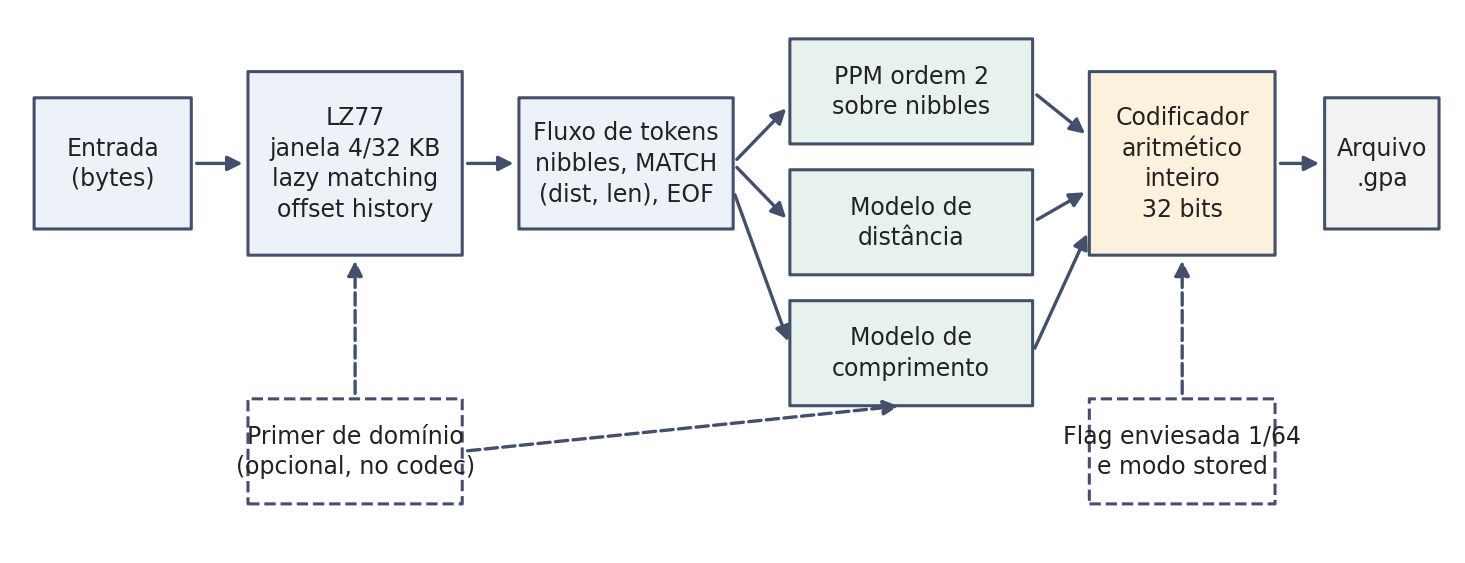
\includegraphics[width=\textwidth]{figs/fig1_pipeline.png}
\caption{Pipeline do GhostPredict. O primer e o modo de armazenamento direto,
  tracejados, são opcionais ao caminho principal.}
\label{fig:pipeline}
\end{figure}

\subsection{Estágio LZ77}

O estágio LZ77 usa janela deslizante de 4~KB no perfil de micro-payload e de
32~KB no perfil de fluxo, comprimento mínimo de casamento de 4 bytes e máximo de
67, busca por cadeia de \textit{hash} de 3 bytes com profundidade máxima de 128
candidatos, e casamento preguiçoso de um passo, que adia a emissão de um
casamento quando a posição seguinte oferece um casamento maior. As distâncias
são quantizadas em 16 faixas de crescimento geométrico, cobrindo de 1 a 32768: o
índice da faixa é codificado pelo modelo adaptativo de distância e o refinamento
dentro da faixa é emitido como bits crus, de 0 a 14 conforme a faixa. Os
comprimentos seguem o mesmo esquema com 7 faixas, de 4 a 67, e de 0 a 5 bits de
refinamento.

Duas memórias curtas completam o estágio e capturam a regularidade de
telemetria. Um histórico das três últimas distâncias, mantido por movimentação
para a frente, permite codificar uma distância repetida como um único símbolo,
sem bits de refinamento; o último comprimento usado recebe o mesmo tratamento.
Em mensagens de estrutura fixa, nas quais os mesmos deslocamentos se repetem a
cada registro, esses dois mecanismos respondem por parte do ganho.

\subsection{Modelagem estatística}
\label{sec:modelagem}

O modelo principal é uma predição por casamento parcial de ordem 2 sobre
nibbles. Cada byte literal é dividido em dois nibbles de 4 bits, e o contexto de
predição é o par de nibbles anterior, o que dá 256 contextos possíveis sobre um
alfabeto de 18 símbolos: os 16 nibbles, um marcador de fim e um marcador de
casamento.

Seja $S$ o contexto corrente, $c(S,X)$ o contador do símbolo $X$ nesse contexto
e $T(S) = \sum_X c(S,X)$ o total acumulado. Num contexto já visitado, o símbolo
$X$ com $c(S,X) > 0$ é codificado com probabilidade

\begin{equation}
P(X \mid S) = \frac{c(S,X)}{T(S) + 1},
\end{equation}

e a probabilidade restante, $1/(T(S)+1)$, fica reservada ao símbolo de escape,
na convenção do método A \cite{cleary:84}. Quando o escape ocorre, o
símbolo é codificado por um modelo de ordem zero com exclusão: os símbolos já
presentes em $S$ são removidos da distribuição de ordem zero, pois não podem ter
causado o escape, o que concentra a probabilidade nos candidatos restantes. Se
$E(S)$ é o conjunto de símbolos com contador positivo em $S$, e $c_0(X)$ o
contador de ordem zero, o símbolo é codificado com

\begin{equation}
P_{\text{esc}}(X \mid S) = \frac{c_0(X)}{\sum_{Y \notin E(S)} c_0(Y)}.
\end{equation}

Após cada símbolo codificado ou decodificado, os contadores do contexto e da
ordem zero são incrementados, nessa ordem exata nos dois lados do canal. Quando
o total de um contexto alcança 2048, todos os seus contadores são divididos por
dois, preservando o mínimo de um. Esse teto permite armazenar o modelo em
contadores de 16 bits, o que reduz o conjunto de trabalho do decodificador aos
19.692 bytes medidos na Seção~\ref{sec:embarcado}.

A escolha de nibbles em vez de bytes segue o mesmo orçamento. Com 256 contextos
de 18 símbolos, o grafo do modelo ocupa cerca de 18~KB, enquanto um modelo de
ordem 2 sobre bytes exigiria $256^2 \times 257$ contadores, na casa de dezenas
de megabytes, inviável no hardware alvo. O preço é codificar dois símbolos por
byte literal, o que aproximadamente dobra o número de operações de codificação
por byte. A Seção~\ref{sec:discussao} retoma esse compromisso.

\subsection{Codificação aritmética inteira}

O codificador mantém um intervalo $[\ell, h]$ de 32 bits e o estreita a cada
símbolo, proporcionalmente à probabilidade que os modelos atribuem. Para um
símbolo com contagem acumulada entre $lo$ e $hi$ sobre um total $t$, a
atualização é

\begin{equation}
r = h - \ell + 1, \qquad
h' = \ell + \left\lfloor \frac{r \cdot hi}{t} \right\rfloor - 1, \qquad
\ell' = \ell + \left\lfloor \frac{r \cdot lo}{t} \right\rfloor ,
\end{equation}

com divisão inteira truncada. Quando os extremos do intervalo passam a concordar
no bit mais significativo, esse bit é emitido e o intervalo é expandido; o caso
de convergência central é tratado com a contagem de bits pendentes descrita
em \cite{witten:87}. O custo de codificar um símbolo de probabilidade $p$
aproxima o limite de $-\log_2 p$ bits. É essa capacidade de gastar frações de
bit que sustenta o desempenho em saídas de dez a vinte bytes, regime no qual
codificadores de bits inteiros desperdiçam margem mensurável.

\subsection{Garantia de não expansão}

O arquivo é apenas o fluxo aritmético, sem cabeçalho, mas a primeira decisão
codificada nesse fluxo é uma escolha binária enviesada entre o modo normal e um
modo de armazenamento direto, com probabilidades $63/64$ e $1/64$. O custo dessa
decisão no caminho comprimido é

\begin{equation}
-\log_2\left(\frac{63}{64}\right) \approx 0{,}023 \text{ bit},
\end{equation}

valor que não altera o tamanho em bytes de nenhum payload do nicho. Quando a
compressão expandiria a entrada, o codificador escolhe o modo de armazenamento,
paga $\log_2 64 = 6$ bits pela decisão, e codifica cada byte por um modelo plano
de 257 símbolos, ao custo de $\log_2 257 \approx 8{,}006$ bits por byte, um
excesso de 0,07\%. Somadas a decisão inicial, a folga por byte e a finalização
do fluxo, a expansão fica limitada a cerca de 0,1\% mais poucos bytes, e o
codificador emite sempre o menor dos dois resultados.

\subsection{Modo com prior}
\label{sec:primed}

O modo com prior está ilustrado na Figura~\ref{fig:sequencia}. Antes de
codificar a mensagem, compressor e descompressor percorrem um corpus de domínio,
o primer, atualizando os modelos de forma idêntica, sem emitir bits, e o utilizam
como dicionário do LZ77: os casamentos da mensagem podem referenciar substrings
do primer. O primer reside no codec e é distribuído uma vez junto ao firmware;
não acompanha mensagem alguma. Cada arquivo permanece sem dicionário, e o ganho
do prior se soma à ausência de custo fixo do formato.

A contrapartida é a dependência de versão: um arquivo só é decodificável com o
mesmo primer usado na compressão, byte a byte. Essa propriedade é compartilhada
com qualquer esquema de dicionário externo e é discutida na
Seção~\ref{sec:discussao}.

\begin{figure}[ht]
\centering
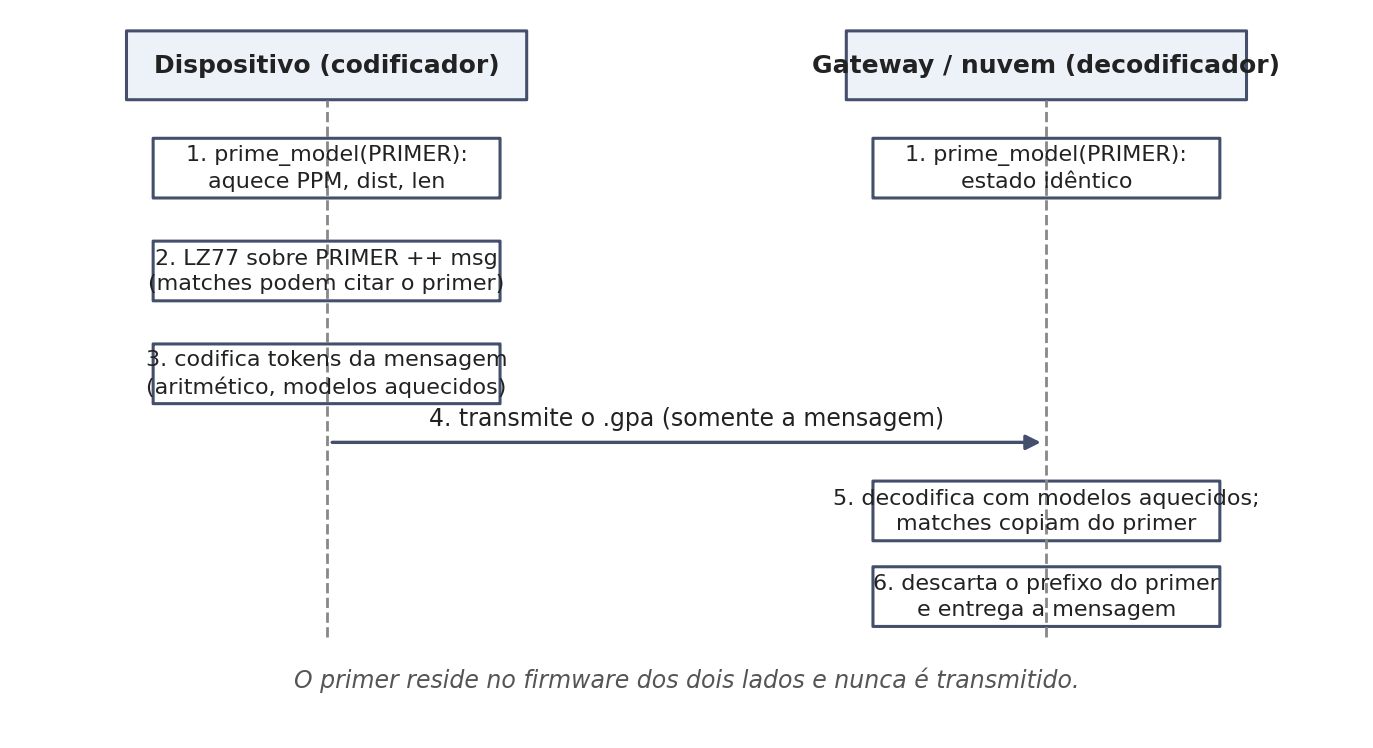
\includegraphics[width=0.92\textwidth]{figs/fig2_sequencia.png}
\caption{Sequência do modo com prior. Os dois lados aquecem o modelo com o mesmo
  primer e chegam a estados idênticos; o arquivo transmitido contém apenas a
  mensagem.}
\label{fig:sequencia}
\end{figure}

% ======================================================================
\section{Metodologia de desenvolvimento}
\label{sec:metdev}

\subsection{Processo dirigido por especificação e por medição}

O projeto seguiu um processo organizado em três artefatos que se verificam
mutuamente.

O primeiro é a especificação algorítmica, independente de linguagem, que define
constantes, modelos, ordem de atualização e formato com precisão suficiente para
que duas implementações desenvolvidas separadamente produzam fluxos bit a bit
idênticos.

O segundo é o conjunto de implementações: um protótipo em Python, usado para
explorar o espaço de projeto; o motor de referência em Rust, sem dependências
externas, que executa compressão e descompressão; e um decodificador em C sem
alocação dinâmica, portado para o ambiente ESP-IDF. As três produzem fluxos
idênticos para as mesmas entradas, o que constitui a verificação cruzada mais
forte disponível ao projeto: um erro de interpretação da especificação em uma
delas apareceria como divergência de bytes.

O terceiro é a suíte de conformidade, com vetores de referência fixos, do
arquivo vazio a padrões repetitivos e dados incompressíveis, que exige
reconstrução bit a bit exata e verifica a garantia de não expansão a cada
alteração do código.

\subsection{Evolução do formato e decisões revertidas}

A evolução foi incremental, com cada versão avaliada pelo mesmo harness de
benchmark com sementes fixas, e decisões desfeitas quando a medição as
contrariou. A Tabela~\ref{tab:versoes} resume a trajetória.

\begin{table}[ht]
\centering
\caption{Evolução do algoritmo. Cada versão foi validada pela suíte de
  conformidade antes de ser incorporada.}
\label{tab:versoes}
\small
\begin{tabular}{ll}
\toprule
\textbf{Versão} & \textbf{Mudança principal} \\
\midrule
v7 & PPM ordem 2 sobre nibbles, com escape e exclusão \\
v8 & Estágio LZ77, janela de 4~KB, faixas de distância e comprimento \\
v9 & Histórico de distâncias, último comprimento, casamento preguiçoso \\
v10 a v10.3 & Pipeline em fluxo; janela de 32~KB; decisão de modo revertida \\
v11 & Modo com prior embutido no codec \\
v11.x & Modelo em contadores de 16 bits; decodificador de 37~KB para 19~KB \\
v12 & Decisão de modo enviesada e modo de armazenamento; contêiner de fluxo \\
v12.1 & Perfil micro com tabelas LZ menores; compressor de 99~KB para 51~KB \\
\bottomrule
\end{tabular}
\end{table}

O exemplo mais ilustrativo do processo é a decisão de modo. Ela foi introduzida
na versão 10 com custo de um bit inteiro, e removida na versão 10.3 porque esse
bit taxava justamente os micro-payloads que motivam o projeto, aumentando em um
byte a saída de oito dos nove casos de referência. Retornou na versão 12 na
forma enviesada descrita na Seção~\ref{sec:algoritmo}, cujo custo de 0,023 bit
preservou o desempenho no nicho e devolveu a garantia de não expansão. A
migração dos contadores de 32 para 16 bits, na versão 11.x, seguiu o mesmo
critério: foi aceita por ser neutra na saída, isto é, por produzir arquivos bit
a bit idênticos, reduzindo o modelo à metade.

\subsection{Arquitetura de software}

A arquitetura do motor está resumida na Figura~\ref{fig:uml}. São seis
componentes com papéis delimitados: o motor central mantém os três modelos
probabilísticos e implementa os caminhos de compressão e descompressão, com e
sem prior; o estágio LZ77 encapsula a busca de casamentos e emite tokens por
retorno de chamada, sem materializar o fluxo em memória; o par de codificador e
decodificador aritméticos realiza a aritmética de intervalo; e o par de escrita
e leitura de bits isola o acesso ao fluxo.

A simetria entre os dois lados é uma invariante de projeto. Toda atualização de
modelo existe em uma única função, chamada de forma idêntica pelos caminhos de
compressão e de descompressão, o que elimina por construção a principal fonte de
dessincronização em codecs adaptativos, que é a divergência entre o aprendizado
do codificador e o do decodificador.

\begin{figure}[ht]
\centering
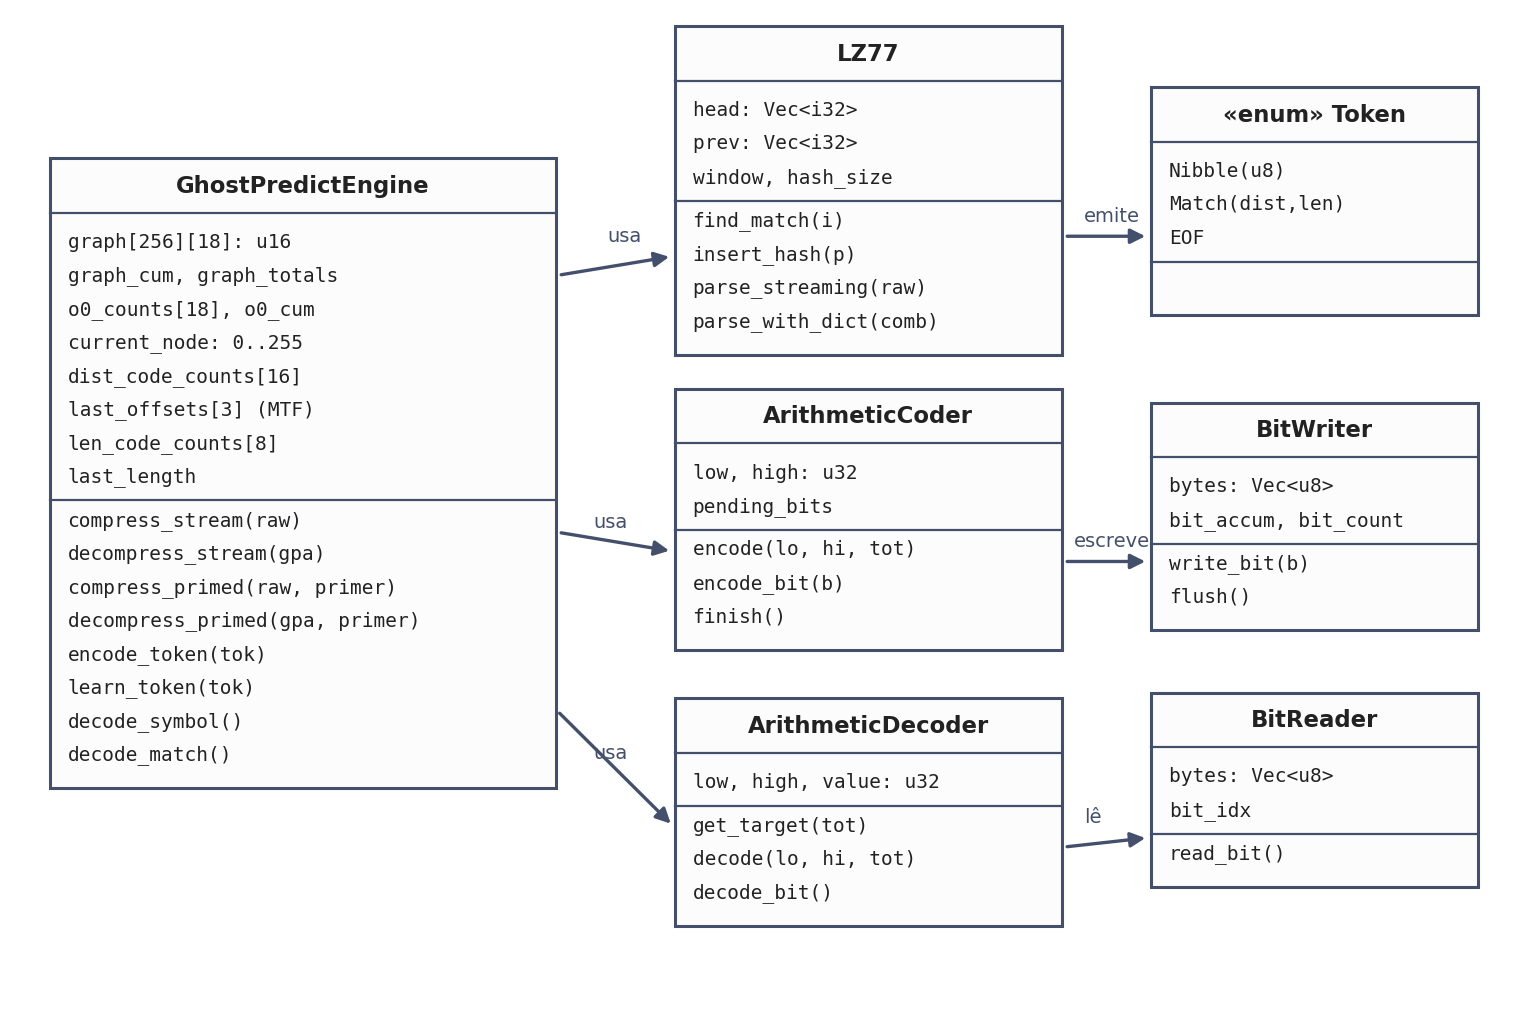
\includegraphics[width=\textwidth]{figs/fig3_uml.png}
\caption{Diagrama de classes do motor de referência em Rust. As setas indicam
  dependência de uso.}
\label{fig:uml}
\end{figure}

% ======================================================================
\section{Metodologia experimental}
\label{sec:metexp}

A avaliação usa onze conjuntos de dados reais, listados na
Tabela~\ref{tab:datasets}, todos tratados como fluxos de registros curtos com um
registro por linha. Para cada domínio, os registros são embaralhados com semente
fixa e divididos em treino e teste disjuntos. O conjunto de treino constrói
tanto o primer do GhostPredict, formado pelos últimos 32~KB do corpus de treino,
quanto o dicionário do zstd, treinado com as mesmas amostras. Os orçamentos,
porém, diferem: o dicionário do zstd foi limitado a 16~KB, metade do primer.
Essa assimetria pode favorecer o GhostPredict, e a comparação com orçamentos iguais
fica como trabalho futuro.

O conjunto de teste, com mil mensagens não vistas por domínio, é comprimido
mensagem a mensagem. Medir mensagens individuais, e não arquivos inteiros, é
uma decisão metodológica central: medir arquivos diluiria o custo de partida a
frio e esconderia o efeito que o prior corrige. A exceção de tamanho são os
quatro conjuntos de log, na versão amostrada de duas mil linhas do Loghub, na
qual teste e treino têm mil mensagens cada.

\begin{table}[ht]
\centering
\caption{Conjuntos de dados reais utilizados na avaliação.}
\label{tab:datasets}
\begin{tabular}{lll}
\toprule
\textbf{Domínio} & \textbf{Fonte} & \textbf{Registro típico} \\
\midrule
MQTT / IoT & MQTTEEB-D \cite{aqachtoul:25} & 76 B \\
AIS / navios & MarineCadastre \cite{marinecadastre:25} & 100 B \\
Sensores & Intel Lab Data \cite{bodik:04} & 64 B \\
Energia & UCI Household Power \cite{hebrail:12} & 62 B \\
GPS & GeoLife \cite{zheng:09} & 65 B \\
Logs (4 tipos) & Loghub \cite{zhu:23} & 84 a 300 B \\
SMS & SMS Spam Collection \cite{almeida:11} & 88 B \\
Tweets & Sentiment140 \cite{go:09} & 148 B \\
\bottomrule
\end{tabular}
\end{table}

Comparam-se dez configurações: o GhostPredict sem prior e com prior; os
especialistas de string curta Unishox2 e SMAZ \cite{sanfilippo:smaz}; o gzip nível 9; o zstd nível 19,
com e sem dicionário treinado; uma variante enxuta do dicionário do zstd, sem
soma de verificação e sem identificador de dicionário, que remove o
enquadramento removível para isolar a contribuição do modelo; o brotli nível 11;
e o xz nível 9. As versões utilizadas foram zstd 1.5.7, xz 5.6.3, gzip 1.13,
brotli 1.1.0 e Unishox2 da distribuição oficial.

As métricas são o tamanho médio, a mediana e o percentil 95 por mensagem, a
fração de mensagens expandidas, a fração de mensagens em que cada ferramenta
produz o menor resultado, a vazão e o uso de memória. O procedimento é
reproduzível a partir do repositório público, com sementes fixas. O repositório
inclui o script de avaliação, com um modo rápido de sanidade, o gerador de
primer, e o decodificador de referência em C verificado bit a bit e medido no
ESP32.

% ======================================================================
\section{Resultados}
\label{sec:resultados}

\subsection{Tamanho por mensagem}

A Tabela~\ref{tab:principal} traz o tamanho médio do comprimido, em bytes, por
domínio e configuração. A Figura~\ref{fig:resultados} apresenta os mesmos dados
para as quatro configurações principais.

\begin{table}[ht]
\centering
\caption{Tamanho médio do comprimido por mensagem, em bytes. Menor é melhor.}
\label{tab:principal}
\small
\begin{tabular}{lrrrrrrrr}
\toprule
\textbf{Domínio} & \textbf{orig} & \textbf{GPA} & \textbf{GPA} &
\textbf{unish.} & \textbf{smaz} & \textbf{zstd} & \textbf{zstd} &
\textbf{brotli} \\
 & & \textbf{frio} & \textbf{prior} & & & \textbf{dict} & \textbf{lean} & \\
\midrule
MQTT (IoT) & 75,33 & 47,71 & \textbf{17,66} & 39,85 & 97,1 & 41,56 & 33,56 & 52 \\
AIS (navios) & 101,02 & 82,89 & \textbf{44,1} & 66,15 & 140,57 & 68,53 & 60,53 & 80,28 \\
Sensores & 63,48 & 48,74 & \textbf{26,08} & 39,21 & 91,02 & 51,87 & 43,87 & 47,63 \\
Medidor & 62,86 & 40,83 & \textbf{17,42} & 36,7 & 81,97 & 39,12 & 31,12 & 39,13 \\
GPS (GeoLife) & 64,95 & 51,3 & \textbf{23,93} & 37,39 & 88,26 & 48,62 & 40,62 & 47,05 \\
Log Apache & 83,51 & 75,14 & \textbf{10,1} & 58,23 & 81,75 & 31,96 & 23,96 & 78,9 \\
Log Linux & 106,89 & 90,29 & \textbf{14,9} & 71,57 & 105,55 & 36,04 & 28,04 & 96,38 \\
Log OpenSSH & 109,38 & 95,78 & \textbf{14,28} & 78,67 & 110,9 & 36,41 & 28,41 & 95,65 \\
Log HDFS & 141,76 & 114,49 & \textbf{32,12} & 94,78 & 151,92 & 53,29 & 45,29 & 117,53 \\
SMS & 80,63 & 66,63 & \textbf{38,99} & 52,72 & 57,48 & 63,91 & 55,91 & 67,01 \\
Tweets & 71,48 & 60,41 & \textbf{35,57} & 46,21 & 47,62 & 60,16 & 52,16 & 60,69 \\
\bottomrule
\end{tabular}
\end{table}

Em todos os domínios o GhostPredict com prior produz o menor arquivo médio.
Sobre o dicionário treinado do zstd, o fator de redução varia de 1,55 a 3,16
vezes, com média 2,12. Esse número inclui o enquadramento do zstd. Contra a
variante enxuta, que remove a soma de verificação e o identificador de
dicionário, o fator cai para 1,37 a 2,37 vezes, com média 1,73, valor que
reflete o modelo. Sobre o Unishox2, especialista sem prior, a média é 2,78
vezes.

\begin{figure}[ht]
\centering
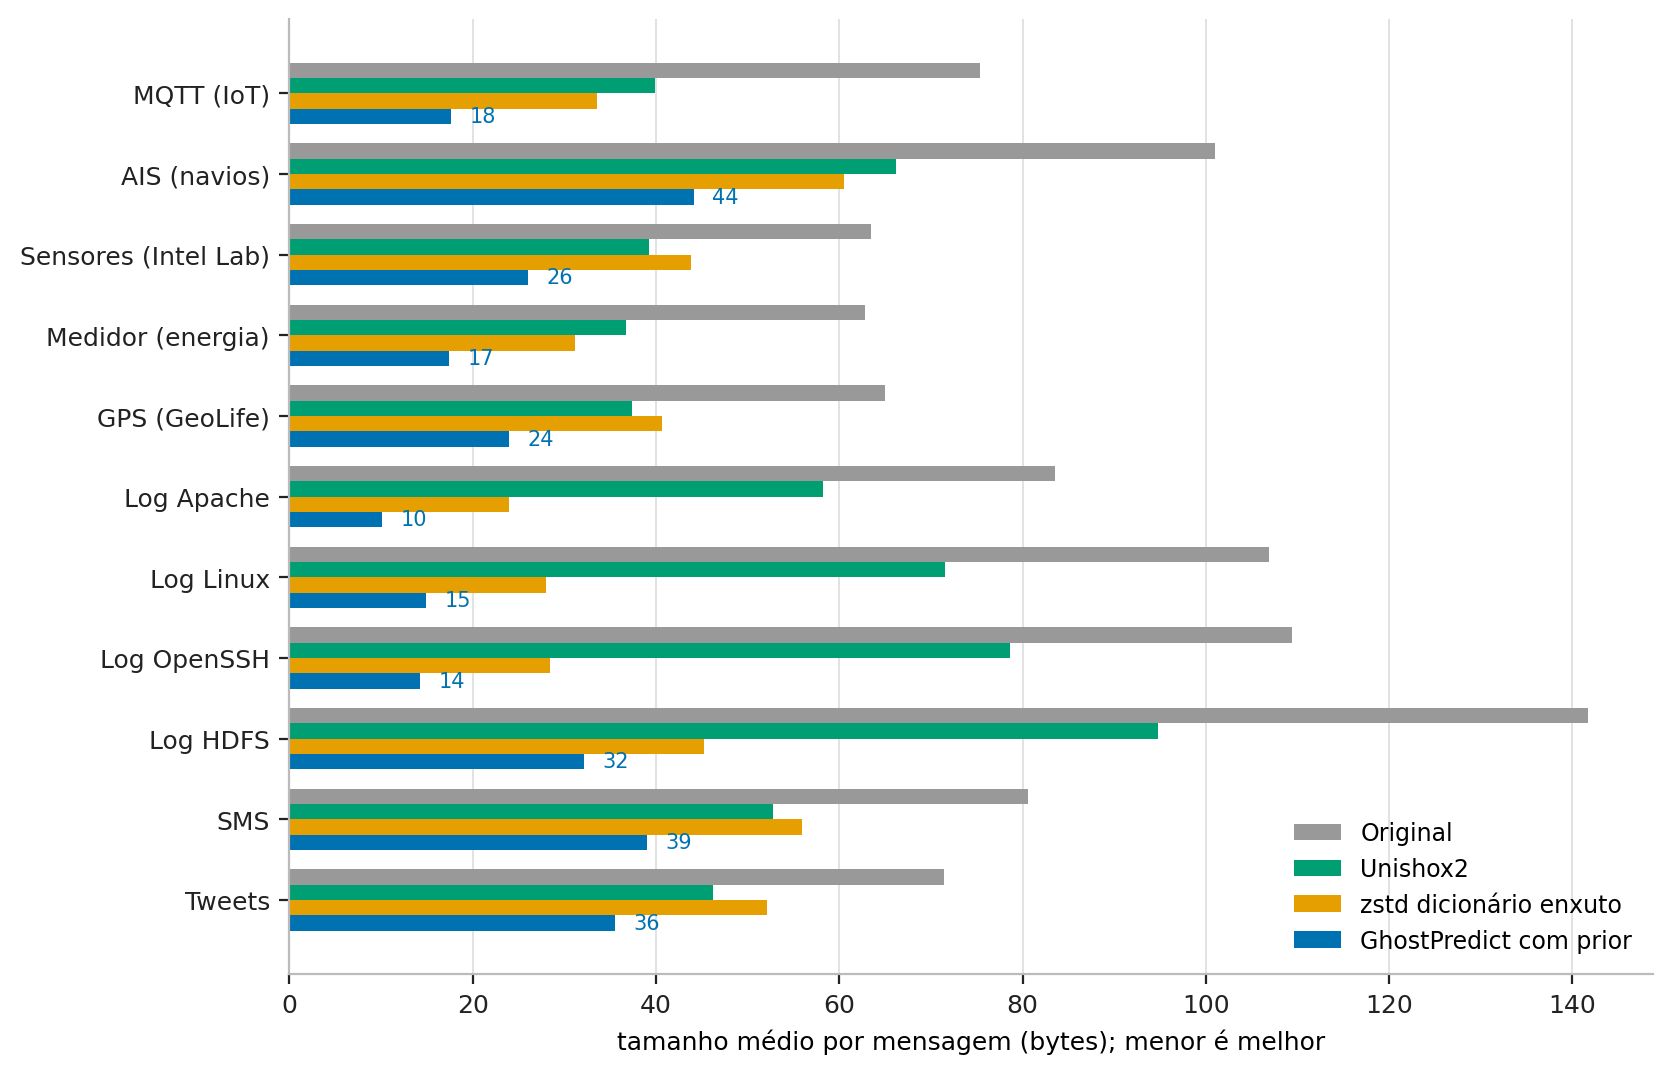
\includegraphics[width=0.95\textwidth]{figs/fig4_resultados.png}
\caption{Tamanho médio por mensagem nas quatro configurações principais.}
\label{fig:resultados}
\end{figure}

\subsection{Decomposição do ganho}
\label{sec:decomp}

A diferença entre as duas comparações acima é o custo fixo de enquadramento.
Medido sobre uma entrada vazia, o dicionário do zstd ocupa 17 bytes na forma
padrão e 9 bytes na forma enxuta, custo que o GhostPredict não paga por não ter
cabeçalho. A Tabela~\ref{tab:decomp} decompõe, em bytes médios por mensagem, a
vantagem sobre o dicionário do zstd em duas parcelas: a moldura removível, que é
a soma de verificação e o identificador de dicionário eliminados pela variante
enxuta, e o restante, que combina o modelo aquecido e o cabeçalho irredutível do
zstd que o formato sem cabeçalho também evita.

\begin{table}[ht]
\centering
\caption{Decomposição da vantagem do GhostPredict com prior sobre o zstd com
  dicionário, em bytes por mensagem.}
\label{tab:decomp}
\begin{tabular}{lrrr}
\toprule
\textbf{Domínio} & \textbf{Vantagem total} & \textbf{Moldura removível} &
\textbf{Modelo e formato} \\
\midrule
MQTT (IoT) & 23,9 & 8 & 15,9 \\
AIS (navios) & 24,4 & 8 & 16,4 \\
Sensores & 25,8 & 8 & 17,8 \\
Medidor (energia) & 21,7 & 8 & 13,7 \\
GPS (GeoLife) & 24,7 & 8 & 16,7 \\
Log Apache & 21,9 & 8 & 13,9 \\
Log Linux & 21,1 & 8 & 13,1 \\
Log OpenSSH & 22,1 & 8 & 14,1 \\
Log HDFS & 21,2 & 8 & 13,2 \\
SMS & 24,9 & 8 & 16,9 \\
Tweets & 24,6 & 8 & 16,6 \\
\bottomrule
\end{tabular}
\end{table}

A moldura removível é constante, de 8 bytes, e a parcela atribuível ao modelo e
ao formato sem cabeçalho varia de 13,1 a 17,8 bytes por mensagem. Ou seja, entre
62\% e 69\% da vantagem permanece depois de conceder ao concorrente o melhor
enquadramento possível.

\subsection{Distribuição dos tamanhos}

A Tabela~\ref{tab:dist} mostra que a vantagem não decorre de poucos casos
extremos: a mediana e o percentil 95 do tamanho por mensagem ficam próximos da
média na maioria dos domínios. As exceções são SMS e Tweets, cuja média excede a
mediana em mais de dez bytes, o que reflete a variabilidade de texto escrito por
pessoas, e não a estrutura fixa da telemetria.

\begin{table}[ht]
\centering
\caption{GhostPredict com prior: média, mediana e percentil 95 do tamanho, em
  bytes.}
\label{tab:dist}
\begin{tabular}{lrrr}
\toprule
\textbf{Domínio} & \textbf{Média} & \textbf{Mediana} & \textbf{P95} \\
\midrule
MQTT (IoT) & 17,66 & 17 & 22 \\
AIS (navios) & 44,1 & 45 & 55 \\
Sensores & 26,08 & 26 & 30 \\
Medidor (energia) & 17,42 & 17 & 21 \\
GPS (GeoLife) & 23,93 & 24 & 31 \\
Log Apache & 10,1 & 10 & 13 \\
Log Linux & 14,9 & 13 & 30 \\
Log OpenSSH & 14,28 & 13 & 23 \\
Log HDFS & 32,12 & 30 & 40 \\
SMS & 38,99 & 28 & 89 \\
Tweets & 35,57 & 33 & 66 \\
\bottomrule
\end{tabular}
\end{table}

\subsection{Expansão e frequência de vitória}

A Tabela~\ref{tab:inflacao} mostra a fração de mensagens que cada ferramenta
expande e a fração em que o GhostPredict com prior produz o menor resultado. Ela
quantifica o problema que motiva o trabalho: no regime de poucas dezenas de
bytes, gzip e xz aumentam o dado na maior parte dos casos, e o xz o faz em
praticamente todos.

\begin{table}[ht]
\centering
\caption{Mensagens expandidas por cada ferramenta e mensagens em que o
  GhostPredict com prior vence, em porcentagem.}
\label{tab:inflacao}
\begin{tabular}{lrrrrr}
\toprule
\textbf{Domínio} & \textbf{GPA prior} & \textbf{gzip} & \textbf{xz} &
\textbf{smaz} & \textbf{unishox2} \\
 & \textbf{vence} & \textbf{expande} & \textbf{expande} & \textbf{expande} &
\textbf{expande} \\
\midrule
MQTT (IoT) & 100 & 54,4 & 100 & 100 & 0 \\
AIS (navios) & 98,9 & 88,1 & 100 & 100 & 0 \\
Sensores & 100 & 100 & 100 & 100 & 0 \\
Medidor (energia) & 100 & 97,6 & 100 & 100 & 0 \\
GPS (GeoLife) & 100 & 93,1 & 100 & 100 & 0 \\
Log Apache & 100 & 100 & 100 & 17,2 & 0 \\
Log Linux & 96,1 & 88,9 & 100 & 47,5 & 0 \\
Log OpenSSH & 99,2 & 79,7 & 100 & 61,9 & 0 \\
Log HDFS & 99,8 & 51 & 99,8 & 97,8 & 0 \\
SMS & 93,9 & 77,5 & 99,2 & 3,9 & 1,1 \\
Tweets & 95,3 & 81,6 & 100 & 2,2 & 0 \\
\bottomrule
\end{tabular}
\end{table}

\subsection{Dependência em relação ao domínio}
\label{sec:cross}

A Tabela~\ref{tab:cross} e a Figura~\ref{fig:cross} quantificam a dependência do
prior em relação ao domínio. Cada célula é o tamanho médio do comprimido, sobre 100 mensagens de teste,
quando se usa o primer do domínio da coluna para comprimir as mensagens de teste do
domínio da linha. A diagonal, com primer casado, é sempre a menor. Fora dela, o
tamanho cresce por um fator de 1,8 a 10,5, e no caso do log do Apache chega a 103 bytes,
acima do tamanho original de cerca de 84 bytes, ou seja, o resultado deixa de
ser compressão.

\begin{table}[ht]
\centering
\caption{Tamanho médio em bytes com primer cruzado. A linha indica o domínio de
  teste e a coluna o domínio do primer.}
\label{tab:cross}
\begin{tabular}{lrrrrr}
\toprule
\textbf{teste / primer} & \textbf{MQTT} & \textbf{AIS} & \textbf{Sensores} &
\textbf{GPS} & \textbf{Log Apache} \\
\midrule
MQTT & \textbf{18,18} & 46,33 & 56,75 & 46,9 & 52,41 \\
AIS & 91 & \textbf{43,21} & 92,16 & 78,25 & 95,91 \\
Sensores & 54,09 & 46,73 & \textbf{26,14} & 47,23 & 50,15 \\
GPS & 49,16 & 42,52 & 51,55 & \textbf{23,71} & 56,24 \\
Log Apache & 99,14 & 97,29 & 102,03 & 103,2 & \textbf{9,82} \\
\bottomrule
\end{tabular}
\end{table}

\begin{figure}[ht]
\centering
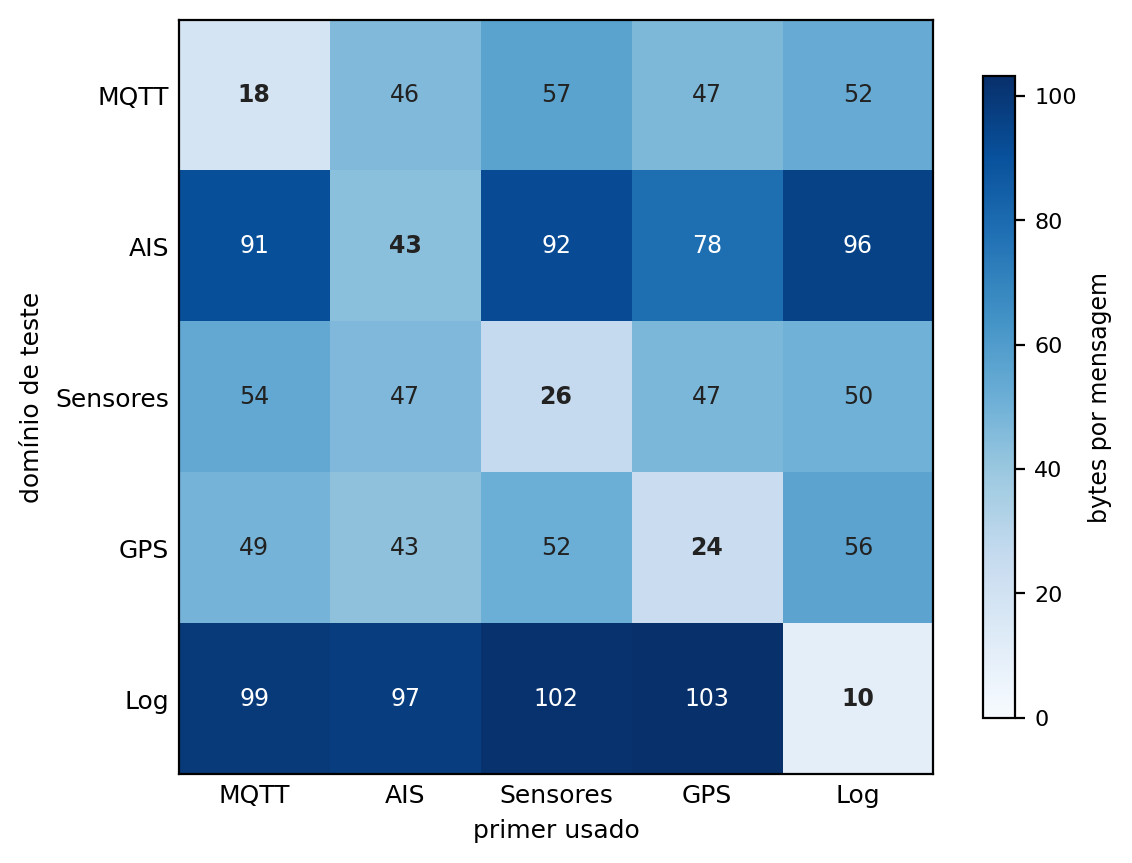
\includegraphics[width=0.72\textwidth]{figs/fig5_cross.png}
\caption{Mapa de calor do experimento cruzado. A diagonal, com primer casado,
  concentra os menores tamanhos.}
\label{fig:cross}
\end{figure}

Este é o limite do método, e o experimento existe para medi-lo em vez de
declará-lo. A Seção~\ref{sec:discussao} discute o que ele implica para
implantação.

\subsection{Vazão e memória}

É preciso separar duas medidas distintas. A Tabela~\ref{tab:vazao} traz a vazão
de compressão e o pico de memória residente do processo no computador de teste,
sobre lotes concatenados. Esse pico inclui o binário e o sistema operacional e
não representa o consumo do algoritmo embarcado. O número relevante para
microcontroladores é o conjunto de trabalho do motor, medido por um alocador
instrumentado e reportado na Seção~\ref{sec:embarcado}.

\begin{table}[ht]
\centering
\caption{Vazão média de compressão e pico de memória do processo no computador
  de teste. Não corresponde ao consumo em microcontrolador.}
\label{tab:vazao}
\begin{tabular}{lrr}
\toprule
\textbf{Configuração} & \textbf{Vazão (MB/s)} & \textbf{Memória do processo (MB)} \\
\midrule
GPA sem prior & 7,0 & 7,1 \\
GPA com prior & 7,2 & 9,3 \\
gzip-9 & 9,8 & 6,6 \\
zstd-19 & 10,0 & 51,9 \\
brotli-11 & 3,1 & 20,5 \\
xz-9 & 4,3 & 42,8 \\
\bottomrule
\end{tabular}
\end{table}

\subsection{Exemplos concretos}

Considere a mensagem MQTT real de 69 bytes reproduzida a seguir, com os campos
intermediários abreviados.

\begin{center}
\texttt{\small 1725866030.472465,0x0018,...,2,dos}
\end{center}

Ela é reduzida pelo GhostPredict com prior a 16 bytes. As demais ferramentas,
sem um prior casado, ficam acima: o
Unishox2 produz 35 bytes, o zstd com dicionário 43 bytes, sua variante enxuta 35
bytes, e o GhostPredict sem prior 42 bytes.

Um exemplo de log esclarece por que os logs comprimem mais. A linha do Apache
\texttt{[Sun Dec 04 06:06:11 2005] [notice] workerEnv.init() ok
/etc/httpd/conf/workers2.properties}, de 91 bytes, é reduzida a 10 bytes, contra
30 bytes do zstd com dicionário, 63 do Unishox2 e 82 do GhostPredict sem prior.
A linha é um molde quase fixo, repetido milhares de vezes no fluxo de log, que o
primer já contém; apenas a parte variável, sobretudo o instante de tempo,
precisa ser codificada. A magnitude dos resultados de log decorre, portanto, da
natureza repetitiva desse tráfego, e não de um artefato de medição.

% ======================================================================
\section{Custo de transmissão e energia em enlaces LPWAN}
\label{sec:energia}

Bytes são um substituto conveniente, mas o orçamento de um dispositivo de campo
é medido em tempo de antena, energia e ciclo de trabalho. Nesta seção
convertemos os resultados da Seção~\ref{sec:resultados} nessas grandezas para um
enlace LoRaWAN, caso em que a conversão tem forma fechada. Em rádios de baixa
potência a transmissão domina o consumo do nó \cite{casals:17}, de modo que a
redução do tempo de antena se traduz de forma quase direta em autonomia.

O tempo de antena de um quadro LoRa é dado pela formulação do transceptor
\cite{semtech:20}. Com fator de espalhamento $SF$, largura de banda $B$ e carga
útil de $PL$ bytes, a duração de um símbolo é $T_s = 2^{SF}/B$, o preâmbulo
padrão custa 12,25 símbolos, e o número de símbolos de payload, com taxa de
código $4/5$, verificação habilitada e cabeçalho explícito, é

\begin{equation}
n_{\text{payload}} = 8 + \max\left(
\left\lceil \frac{8\,PL - 4\,SF + 44}{4\,(SF - 2\,DE)} \right\rceil \cdot 5,\ 0
\right),
\end{equation}

na qual $DE$ vale 1 nos fatores SF11 e SF12, que exigem otimização de taxa
baixa, e 0 nos demais. Ao payload de aplicação somamos os 13 bytes de sobrecarga
mínima de um enlace de subida LoRaWAN, referentes a MHDR, DevAddr, FCtrl, FCnt,
FPort e MIC \cite{loraalliance:18a}. Para a energia de transmissão adotamos
$E = V I T$, com a corrente de 28~mA do transceptor SX1276 transmitindo a
$+13$~dBm e alimentação de 3,3~V \cite{semtech:20}, o que dá potência de
92,4~mW. São estimativas analíticas, não medições; a validação com transceptor
real permanece como trabalho futuro.

A mensagem MQTT média tem 75,33 bytes, o que dá um quadro de 89 bytes com a
sobrecarga do LoRaWAN. Em SF12 com 125~kHz, a duração de símbolo é 32,768~ms e o
quadro ocupa 3,6~s de antena, consumindo cerca de 334~mJ. Comprimida, a mesma
mensagem cai para 17,66 bytes, quadro de 31 bytes, 1,8~s de antena e cerca de
167~mJ. Sob o ciclo de trabalho de 1\% da banda EU868, o orçamento de 36
segundos de antena por hora passa de 9 para 19 mensagens por hora.

\begin{table}[ht]
\centering
\caption{Quadro médio, tempo de antena e energia estimados por mensagem, do
  payload original para o comprimido com prior. SF7 e SF12, 125~kHz, taxa de
  código 4/5, sobrecarga LoRaWAN de 13~B incluída.}
\label{tab:lora}
\small
\begin{tabular}{lrrrrr}
\toprule
\textbf{Domínio} & \textbf{Quadro (B)} & \textbf{SF7 (ms)} & \textbf{SF12 (s)} &
\textbf{Energia SF12 (mJ)} & \textbf{Redução} \\
\midrule
MQTT (IoT) & 89 $\to$ 31 & 154 $\to$ 72 & 3,6 $\to$ 1,8 & 334 $\to$ 167 & 50\% \\
AIS (navios) & 115 $\to$ 58 & 195 $\to$ 113 & 4,4 $\to$ 2,6 & 410 $\to$ 243 & 41\% \\
Sensores & 77 $\to$ 40 & 138 $\to$ 82 & 3,3 $\to$ 2,0 & 304 $\to$ 182 & 40\% \\
Medidor (energia) & 76 $\to$ 31 & 138 $\to$ 72 & 3,3 $\to$ 1,8 & 304 $\to$ 167 & 45\% \\
GPS (GeoLife) & 78 $\to$ 37 & 138 $\to$ 82 & 3,3 $\to$ 2,0 & 304 $\to$ 182 & 40\% \\
Log Apache & 97 $\to$ 24 & 169 $\to$ 62 & 3,9 $\to$ 1,5 & 364 $\to$ 137 & 62\% \\
Log Linux & 120 $\to$ 28 & 200 $\to$ 67 & 4,6 $\to$ 1,6 & 425 $\to$ 152 & 64\% \\
Log OpenSSH & 123 $\to$ 28 & 205 $\to$ 67 & 4,8 $\to$ 1,6 & 440 $\to$ 152 & 65\% \\
Log HDFS & 155 $\to$ 46 & 251 $\to$ 92 & 5,7 $\to$ 2,3 & 531 $\to$ 213 & 60\% \\
SMS & 94 $\to$ 52 & 164 $\to$ 103 & 3,8 $\to$ 2,5 & 349 $\to$ 228 & 35\% \\
Tweets & 85 $\to$ 49 & 149 $\to$ 98 & 3,4 $\to$ 2,3 & 319 $\to$ 213 & 33\% \\
\bottomrule
\end{tabular}
\end{table}

A Tabela~\ref{tab:lora} estende a conta aos onze domínios e a
Figura~\ref{fig:airtime} mostra o efeito em SF12, o fator de maior alcance e
maior custo. A redução de tempo de antena varia de 33\% a 65\% conforme o
domínio.

\begin{figure}[ht]
\centering
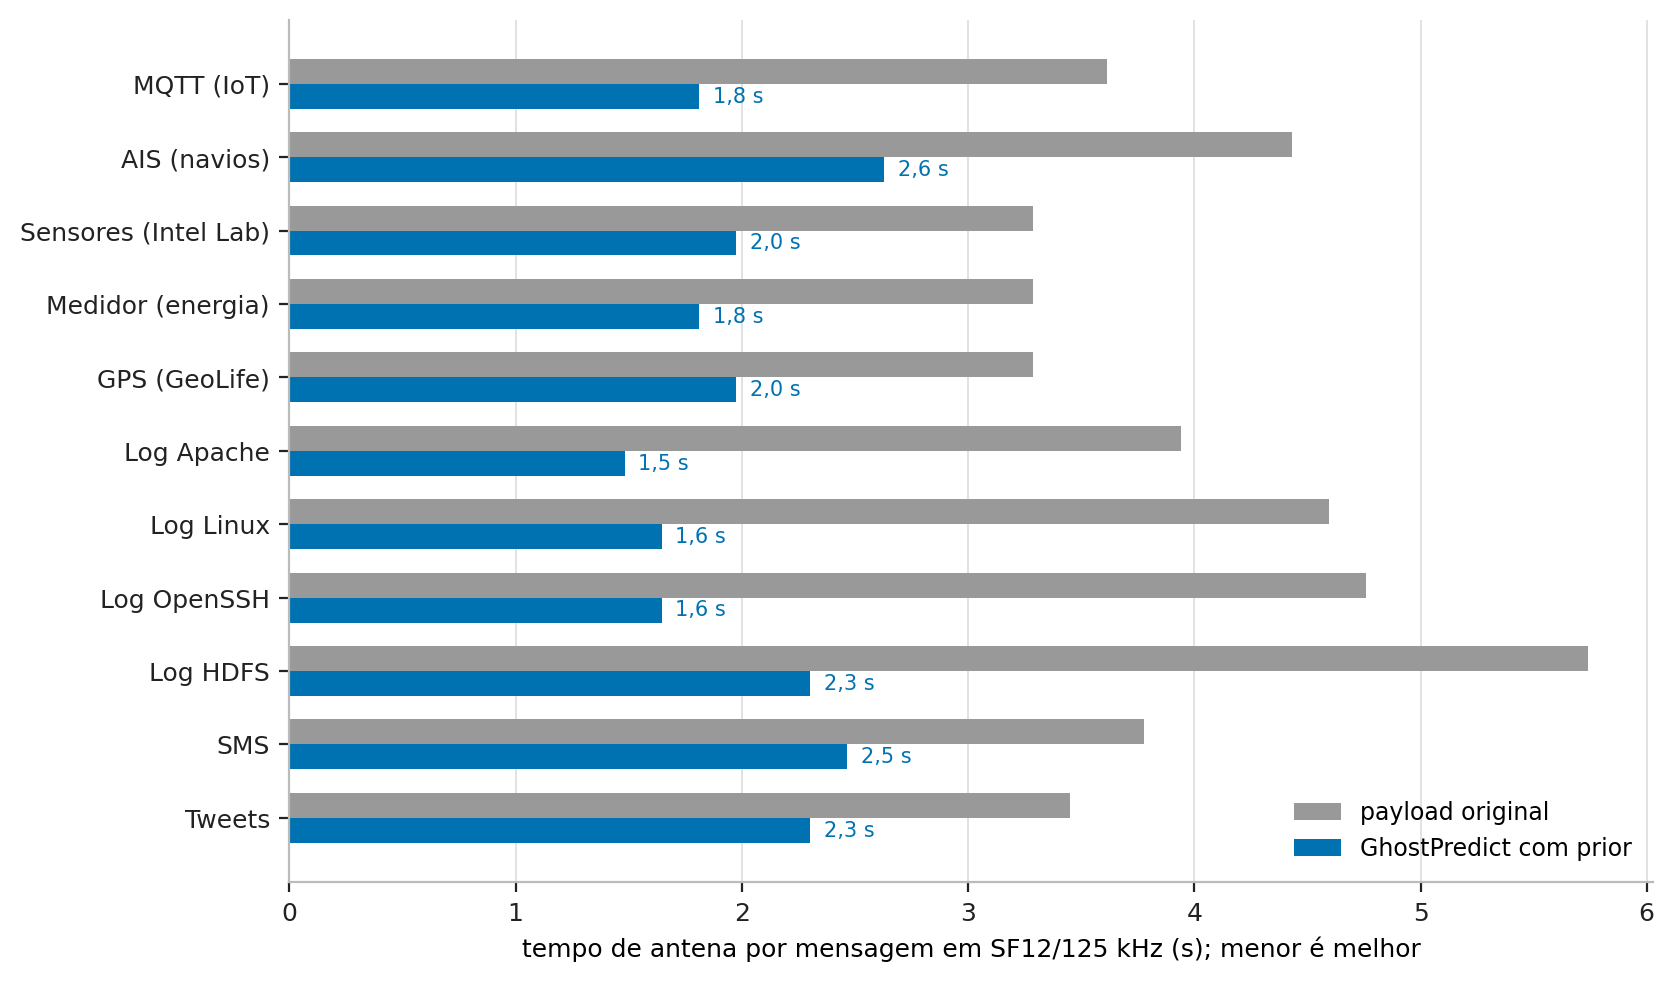
\includegraphics[width=0.95\textwidth]{figs/fig6_airtime.png}
\caption{Tempo de antena estimado por mensagem em SF12 e 125~kHz, antes e depois
  da compressão com prior.}
\label{fig:airtime}
\end{figure}

Há um efeito que a média esconde. Na taxa mais restritiva da banda EU868, DR0,
que corresponde a SF12 com 125~kHz, o payload de aplicação é limitado a 51 bytes
\cite{loraalliance:18b}. A mensagem média original excede esse limite nos onze
domínios avaliados, isto é, no alcance máximo do enlace ela não cabe em um
quadro e exigiria fragmentação na aplicação. Comprimida com prior, a mensagem
média cabe nos onze. Para um dispositivo na borda de cobertura, a compressão
deixa de ser economia e passa a ser condição para transmitir.

% ======================================================================
\section{Validação em hardware embarcado}
\label{sec:embarcado}

\subsection{Arquitetura de uso e método de medição}

O destino do método são dispositivos de recursos restritos, como os
microcontroladores das famílias ESP32, STM32 e nRF. A arquitetura de uso é
assimétrica: o dispositivo comprime a mensagem antes de transmitir, com o
codificador e o primer gravados no firmware, e o gateway ou a nuvem descomprime.
Como todo o pipeline usa apenas aritmética inteira, ele não exige unidade de
ponto flutuante e executa de forma idêntica no microcontrolador e no servidor.

Para medir, portamos o decodificador para C sem alocação dinâmica, com todo o
estado em memória estática, e o verificamos contra o motor de referência nos
vetores de conformidade e em mensagens reais. O firmware executa doze mensagens
de teste retiradas do conjunto de dados, repetindo cada uma 200 vezes no modo
sem prior e 10 vezes no modo com prior, e cronometra com o temporizador de alta
resolução da plataforma. A integridade é verificada por comparação byte a byte
do resultado com a mensagem original a cada repetição. O ambiente foi um
ESP32-D0WDQ6 revisão v1.1, dois núcleos a 240~MHz, com ESP-IDF v5.5.5 e
otimização por tamanho.

\subsection{Resultados medidos}

A Tabela~\ref{tab:esp32} e a Figura~\ref{fig:esp32} reúnem as medições. As 24
execuções, doze em cada modo, reconstruíram a mensagem original bit a bit.

\begin{table}[ht]
\centering
\caption{Medições do decodificador em ESP32-D0WDQ6 a 240~MHz, ESP-IDF v5.5.5,
  sobre doze mensagens de teste.}
\label{tab:esp32}
\begin{tabular}{lrr}
\toprule
\textbf{Métrica} & \textbf{Sem prior} & \textbf{Com prior} \\
\midrule
Compressão média & 58,2 B $\to$ 49,4 B & 58,2 B $\to$ 16,9 B \\
Fator & 1,18 & 3,44 \\
Latência média por mensagem & 698 $\mu$s & 47.665 $\mu$s \\
Latência mediana & 725 $\mu$s & 47.562 $\mu$s \\
RAM estática (.bss) & 19.692 B & 68.852 B \\
RAM dinâmica (heap) & 0 B & 196.844 B \\
RAM total & 19,7 KB & 265,7 KB \\
Flash (código e constantes) & 2.031 B & 3.413 B \\
Reconstrução bit a bit & 12 de 12 & 12 de 12 \\
\bottomrule
\end{tabular}
\end{table}

\begin{figure}[ht]
\centering
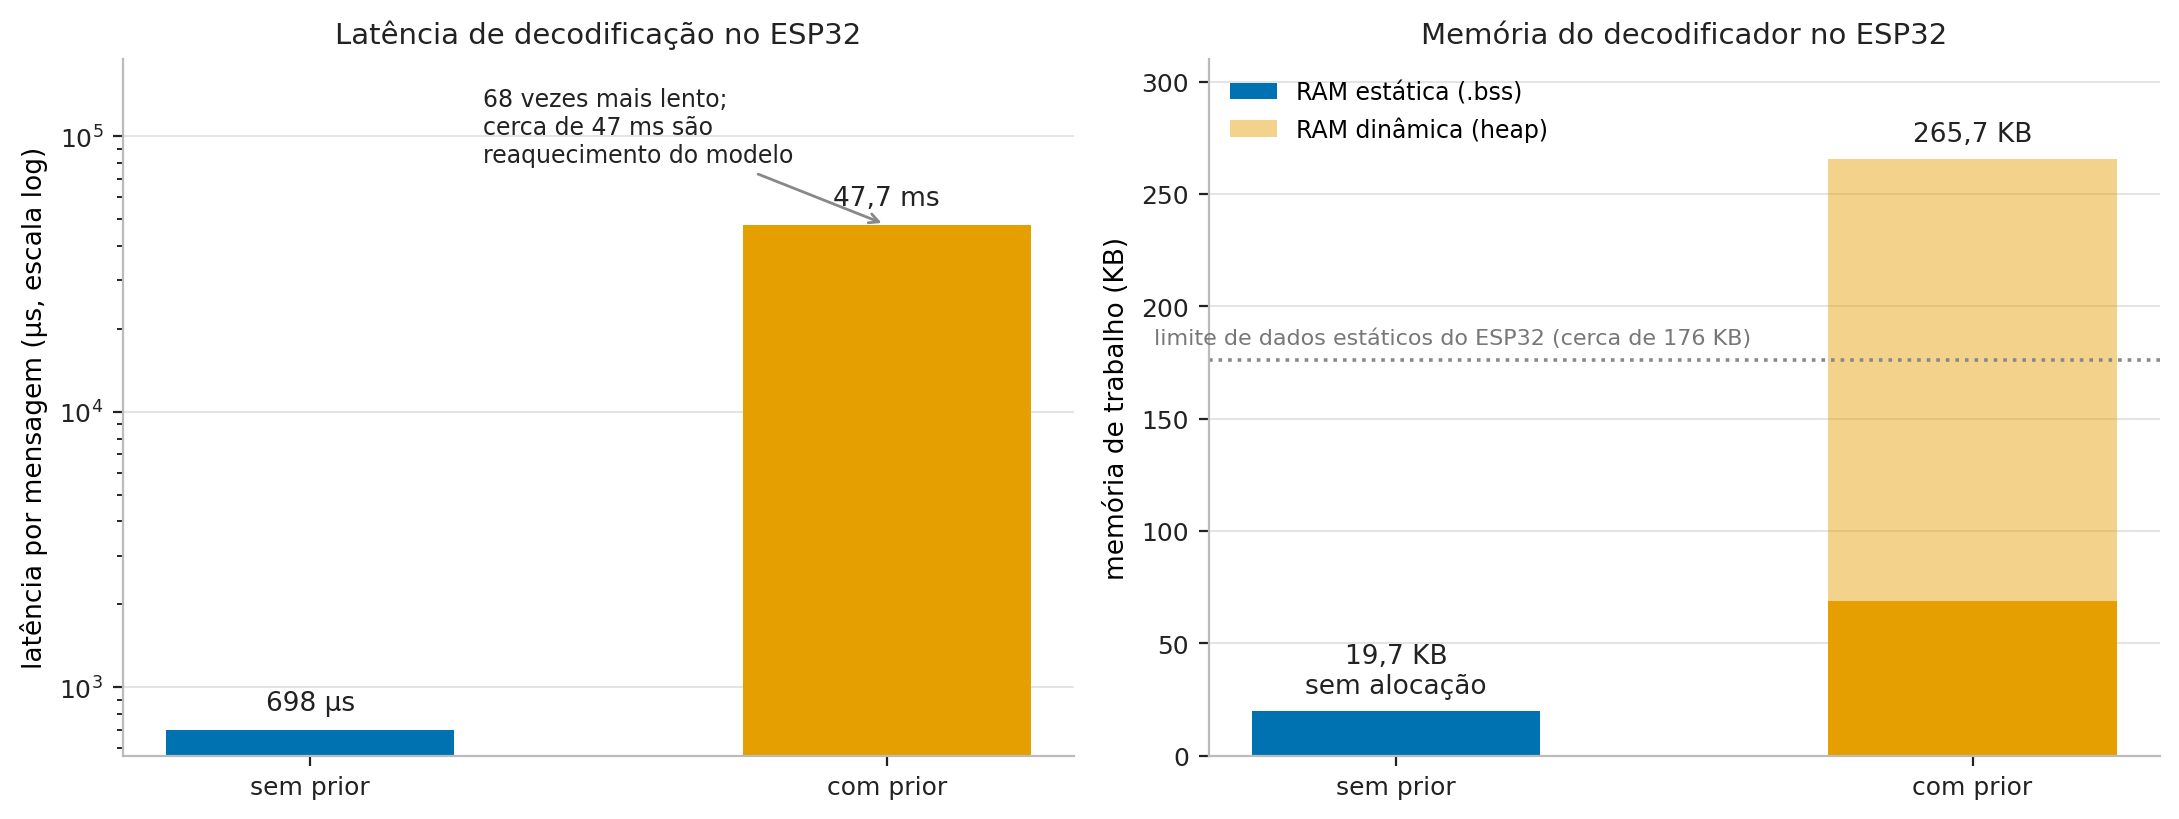
\includegraphics[width=\textwidth]{figs/fig7_esp32.png}
\caption{Latência e memória do decodificador medidas no ESP32. A escala da
  latência é logarítmica.}
\label{fig:esp32}
\end{figure}

O valor de 19.692 bytes de RAM estática no modo sem prior converge com duas
medições independentes obtidas no computador de desenvolvimento, um alocador
instrumentado em Rust, que reportou 19.083 bytes, e a análise do objeto
compilado, que reportou 19.776 bytes. A diferença entre as três está abaixo de
4\% e decorre de alinhamento e de estruturas auxiliares de cada ambiente.

\subsection{O custo do modo com prior}
\label{sec:custoprior}

A medição revelou um custo que a análise estática não antecipava. O modo com
prior consome 47,7~ms por mensagem, 68 vezes o modo sem prior. A decomposição do
tempo mostra que cerca de 47~ms correspondem ao reaquecimento do modelo: o
decodificador reprocessa os 16~KB do primer usado no teste embarcado, metade
dos 32~KB da avaliação da Seção~\ref{sec:metexp}, com o estágio LZ77 e reexecuta o
aprendizado de todos os tokens a cada mensagem, enquanto a decodificação
propriamente dita permanece na casa de centenas de microssegundos.

Duas restrições de memória também apareceram apenas na plataforma real. As
tabelas da cadeia de \textit{hash} do LZ77 somam 192~KB e não cabem no segmento
de dados estáticos do ESP32, limitado a cerca de 176~KB, o que faz a ligação
falhar. A causa não é o subsistema de rádio, mas o tamanho do segmento. A
solução adotada foi alocar essas duas tabelas do heap, que alcança regiões de
memória indisponíveis para dados estáticos, mantendo o caminho sem prior
integralmente estático. Além disso, a ordem de alocação importa: o heap da
plataforma é dividido em regiões, a maior com 157~KB, e solicitar primeiro a
tabela menor, de 64~KB, faz a solicitação seguinte, de 128~KB, falhar por
ausência de bloco contíguo.

Colocado em perspectiva, o custo de processamento ainda é pequeno diante do
custo de rádio. Os 47,7~ms correspondem a 2,7\% do tempo de antena de 1,8~s
estimado para a mensagem MQTT comprimida em SF12. Estimando o consumo de CPU em
40~mA a 3,3~V, o processamento gasta cerca de 6,3~mJ para economizar cerca de
167~mJ de transmissão. O balanço permanece favorável em enlaces de baixa
potência, mas a margem deixa de ser desprezível em enlaces rápidos.

Cabe uma ressalva sobre a direção da medição. O que se mediu foi o
decodificador, enquanto na arquitetura de uso é o dispositivo que comprime. O
compressor executa o mesmo aquecimento e ainda a busca de casamentos da
mensagem, de modo que 47,7~ms constitui um piso, e não o custo do lado do
dispositivo. Portar o compressor para C e medi-lo é trabalho pendente.

% ======================================================================
\section{Discussão}
\label{sec:discussao}

\subsection{Interpretação dos resultados}

Os resultados sustentam a tese e delimitam seu alcance. No nicho de
micro-payloads, o prior embutido no codec entrega o menor arquivo em 94\% a
100\% das mensagens, conforme o domínio. É importante separar as duas fontes
desse ganho. Parte vem do formato sem cabeçalho, pois o dicionário do zstd
carrega um enquadramento fixo que, em saídas de algumas dezenas de bytes,
representa fração relevante. Ao remover o enquadramento removível, a vantagem
cai mas permanece entre 62\% e 69\% do total. A parte restante vem do modelo
aquecido pelo prior. Ambas as fontes são contribuições do método, e a
decomposição evita atribuir ao modelo um ganho que é, em parte, de formato.

\subsection{Limites}

Fora do nicho o método não compete. Em dados de maior porte a razão de
compressão fica próxima à do gzip, atrás de zstd, xz e brotli, pelas razões
identificadas na Seção~\ref{sec:modelagem}: janela curta, modelo de ordem baixa
e alfabeto de nibbles. Em texto de linguagem natural livre, compressores de
caractere permanecem competitivos, como mostram as colunas de SMS e Tweets, nas
quais o SMAZ, que expande quase todas as mensagens de telemetria, expande apenas
3,9\% e 2,2\% das mensagens e se aproxima do Unishox2.

A principal ameaça à validade é a dependência entre o prior e o domínio,
quantificada na Seção~\ref{sec:cross}: um prior de domínio distinto degrada o
resultado por um fator de até 10,5 e pode levar o tamanho comprimido a exceder o
original. A avaliação usa mil mensagens por domínio; uma validação industrial
deveria ampliar amostras e domínios.

Some-se o custo de latência medido na Seção~\ref{sec:custoprior}, que restringe
a aplicabilidade do modo com prior a dispositivos com pelo menos algumas
centenas de quilobytes de RAM disponíveis e a taxas de mensagem compatíveis com
dezenas de milissegundos de processamento por mensagem.

Por fim, os limites próprios de uma prova de conceito. O compressor não foi
portado nem medido no microcontrolador; a energia é estimada analiticamente, sem
instrumento de corrente nem transceptor real; o modo com prior ainda reaquece o
modelo a cada mensagem; não houve avaliação em rede real nem em frota; e a vazão
de cerca de 7~MB/s, adequada a mensagens curtas, não foi otimizada. Esses pontos
separam a demonstração de viabilidade aqui relatada de uma implementação de
produção.

\subsection{Balanço de engenharia}

Estabelecido que o efeito existe e medido de onde ele vem, a questão prática
passa a ser o balanço. A proposta troca um custo fixo por um ganho recorrente. O
custo é o primer, de 16 a 32~KB na memória de programa do dispositivo, pago uma
única vez e nunca transmitido, somado à memória de trabalho da
Tabela~\ref{tab:custos}. O ganho é a redução em cada mensagem enviada.

\begin{table}[ht]
\centering
\caption{Custos do método, com os valores do modo correspondente. Os números do
  modo com prior são os medidos no ESP32.}
\label{tab:custos}
\begin{tabular}{lr}
\toprule
\textbf{Item} & \textbf{Valor} \\
\midrule
Primer, em memória de programa & 16 a 32 KB \\
Decodificador sem prior, RAM de trabalho & 19,7 KB \\
Decodificador com prior, RAM de trabalho & 265,7 KB \\
Compressor sem prior, perfil micro, RAM de trabalho & 51 KB \\
Compressor com prior, RAM de trabalho & cerca de 232 KB \\
Latência do decodificador sem prior, no ESP32 & 698 $\mu$s \\
Latência do decodificador com prior, no ESP32 & 47,7 ms \\
Degradação com primer descasado & até 10,5 vezes \\
\bottomrule
\end{tabular}
\end{table}

Em um cenário de IoT com dispositivo que transmite muitas mensagens curtas por
enlaces onde cada byte custa energia e tempo de antena, o balanço é favorável,
pois a memória de programa investida é abundante nos microcontroladores usuais,
e a economia se acumula a cada transmissão. A condição para que o compromisso
compense é a estabilidade do domínio. O método é indicado quando o domínio é
estável e o volume de mensagens é alto, e contraindicado quando o tráfego é
heterogêneo ou a memória disponível é escassa.

\subsection{Ciclo de vida do primer}

Como um arquivo só é decodificável com o primer exato usado na compressão, a
atualização do prior em uma frota implantada precisa ser tratada como parte do
firmware: o primer é versionado junto com a imagem, distribuído pelo mesmo canal
de atualização remota, e a versão vigente é acordada no nível do protocolo de
aplicação, por exemplo por um identificador curto trocado no estabelecimento da
sessão, fora das mensagens. Essa exigência não é peculiar ao GhostPredict:
qualquer esquema de conhecimento compartilhado, dos dicionários treinados do
zstd às regras de contexto do SCHC \cite{minaburo:20}, impõe a mesma disciplina
de sincronização entre as pontas. A diferença prática é que o primer é um corpus
bruto, gerado por um script determinístico a partir de amostras do próprio
tráfego, o que torna a atualização um processo de dados, sem alteração de
código.

\subsection{Ganhos do estudo}

Além do compressor, o trabalho produziu resultados de método que se aplicam além
dele.

O procedimento de decomposição do ganho, que separa a parcela de formato da
parcela de modelo por meio de uma variante enxuta do concorrente, é
generalizável a qualquer comparação entre um formato sem cabeçalho e um formato
enquadrado, e evita uma atribuição de mérito que seria incorreta.

O experimento cruzado estabelece um procedimento para medir a fragilidade de
métodos baseados em conhecimento prévio, em vez de apenas declará-la como
limitação. O resultado, uma degradação de até 10,5 vezes, é informação
acionável para quem for implantar.

A verificação por três implementações independentes com saída bit a bit idêntica
mostrou-se o instrumento mais eficaz de validação do projeto, superior à suíte
de testes de uma única implementação, por detectar erros de interpretação da
especificação e não apenas erros de código.

Por fim, a medição em hardware real corrigiu duas conclusões que a análise
estática havia sugerido: o consumo de memória do modo com prior excede o
segmento de dados estáticos da plataforma, e o custo de latência desse modo é
cerca de 68 vezes maior que o do modo sem prior. Nenhum dos dois efeitos
era visível sem executar no dispositivo, o que reforça o valor da validação em
plataforma real em trabalhos desta natureza.

% ======================================================================
\section{Conclusão e trabalhos futuros}

Apresentamos o GhostPredict, uma prova de conceito de compressor sem perdas para
micro-payloads de IoT que combina formato sem cabeçalho, garantia de não expansão a um custo de 0,023
bit, e um prior de domínio embutido no codec. A avaliação em onze conjuntos de
dados reais mostra que, no seu nicho, o método produz o menor arquivo em 94\% a
100\% das mensagens, e que, isolando o modelo do formato, mantém fator médio de
1,73 sobre o dicionário treinado do zstd em sua forma mais enxuta, preservando
arquivos sem dicionário. A análise de enlace mostra redução de 33\% a 65\% no
tempo de antena e na energia de transmissão em LoRaWAN, e que a mensagem média
dos onze domínios só cabe na taxa mais restritiva depois de comprimida. A
medição em ESP32 confirma o consumo de 19.692 bytes de RAM no modo sem prior,
com latência de 698 microssegundos por mensagem, e quantifica em 47,7
milissegundos o custo do modo com prior. Os ganhos dependem da existência de um
prior compatível com o domínio, condição quantificada na
Seção~\ref{sec:cross}. Em conjunto, os resultados confirmam a hipótese que
motivou a prova de conceito: compartilhar o prior no codec, e não no arquivo, é
vantajoso para micro-payloads.

Os trabalhos futuros, que levam a prova de conceito a uma implementação de
produção, seguem quatro frentes.

A primeira, decorrente do resultado da Seção~\ref{sec:custoprior}, é substituir
o reaquecimento por mensagem por um estado de modelo pré-computado. O estado
resultante do aquecimento é determinístico e ocupa cerca de 19,7~KB, de modo que
pode ser calculado fora do dispositivo e gravado em memória de programa, sendo
restaurado por cópia antes de cada mensagem. Nesse desenho o decodificador
dispensa as tabelas do LZ77, o que reduziria a memória de 265,7~KB para cerca de
36~KB e a latência para a ordem do modo sem prior. É a mudança de maior impacto
identificada pelo trabalho.

A segunda é medir o compressor no dispositivo, e não apenas o decodificador,
para fechar a lacuna apontada na Seção~\ref{sec:custoprior}, e medir a energia
com instrumento de corrente e transceptor LoRa, substituindo as estimativas
analíticas da Seção~\ref{sec:energia}.

A terceira é o modelo: um contexto de ordem mais alta, ou uma mistura de
contextos, deve reduzir o custo de codificação, ao preço de memória. O ponto de
equilíbrio em microcontroladores é uma questão em aberto, e a análise da
Seção~\ref{sec:modelagem} indica que o alfabeto de nibbles é o principal fator
limitante do modelo atual.

A quarta é operacional: formalizar o protocolo de versionamento e atualização do
primer em frotas, ampliar os domínios e o número de amostras da avaliação, e
incluir mais especialistas de string curta na comparação, e repetir a comparação
com o zstd usando dicionário do mesmo tamanho do primer.

\bibliographystyle{sbc}
\bibliography{refs}

\end{document}
